\documentclass{article}
\usepackage{graphicx}
\usepackage{float}
\usepackage{svg}
\def \scalingfactor{.8}

\begin{document}

\title{Benchmarking Fermi Microarchitecture}
\author{Paolo Ienne, Andrea Miele\and Ewaida Moshen, Cl\'{e}ment Humbert, Tristan Overney}
\date{\today}
\maketitle

\section{Goals}
	The goals of this benchmarking is to expose the Fermi microarchitecture details
    as implemented in Nvidia Fermi cards (pipeline length, instructions latency,
    scheduling patterns, etc.) in order to know what can and cannot be changed
    to create an integer computation oriented device.

\section{Methods}
	To achieve the aforementioned goals, a serie of specially crafted CUDA kernels
	were used. These usually contain large batches of dependent instructions that were 
	timed with the assistance of the \texttt{clock64()} function offered by the CUDA API.

	The benchmark programs have been ran on a machine equipped with an Nvidia
    GeForce GTX 580 GPU.

\section{Terminology}
    Before diving into the experiments and their results here's a quick-start
    guide to Nvidia's Fermi architecture and its vocabulary:

    \subsection{Streaming Multiprocessors}
    The largest building block inside the Fermi architecture is the 
    \emph{Streaming multiprocessor} (Figure ~\ref{fig:SM} on page 
    ~\pageref{fig:SM}) abbreviated SM in this report. Fermi cards are equipped
    with 16 of these SMs.
    \begin{figure}[H]
    \centering
        \includesvg[width=\scalingfactor\linewidth]{FermiSM}
        \caption{Fermi's streaming multiprocessor schematic representation}
        \label{fig:SM}
    \end{figure}

    Each SM is composed of the following computation blocks:
    \begin{itemize}
        \item 32 CUDA cores in two groups of 16,
        \item 16 load/store units (LD/ST on the figure)
        \item 4 Special Functions Units (SFUs) dedicated to more complex
              arithmetic functions such as sines and logarithms.
    \end{itemize}
    
    As the SFUs are dedicated to floating-point operations they're already an
    area that can be reused for integer computation components, thus it's not
    part of the following research. The focus of the experiments are the 
    CUDA cores.

    \subsection{CUDA Cores}
    Figure~\ref{fig:CUDACore} is the representation of what a CUDA core is,
    according to Nvidia.
    
    \begin{figure}[H]
    \centering
        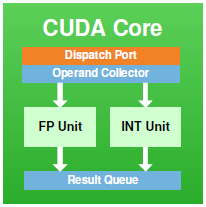
\includegraphics{pictures/CUDACore}
        \caption{Schematic representation of Nvidia's CUDA Core}
        \label{fig:CUDACore}
    \end{figure}
    
    From figure~\ref{fig:CUDACore} the notion of twice 16 cores can be 
    extended to twice 16 integers ALUs and 16 simple-precision floating-point
    ALUs. The interesting parts are the "FP Unit" and "INT Unit" as the rest
    can be left as-is.

\section{Pipeline properties}
	This section contains the results obtained through the previously described
	methods using large batches of integer multiplications.

	\subsection{Benchmark running times against number of threads}
	\label{sectiondassaut}
	\subsubsection{Description of the experiment}
	The following experiment is trying to outline the relation between the running
    times of the benchmark program and the number of threads running parallely in
    a single block (i.e.: the threads reside on one SM).
	\subsubsection{Expectations}
    The running times are expected to be slightly higher for the integer
    multiplications but to deteriorate in a similar fashion (begin to deteriorate
    at the same point, at the same rate) due to each core being equipped with
    integer and single-precision floating-point ALUs.
	\subsubsection{Results and analysis}
    \begin{figure}[h]
    	\centering
		\vspace{-20pt}
        % TODO: replace with graphic containing both INT and FP results
	    \includegraphics[width=\scalingfactor\linewidth]{"graphics/running_times"}
		\vspace{-15pt}
        \caption{Running times of benchmark (in cycles) against number of threads}
    \end{figure}
	\pagebreak
    
    \subsubsection{Results}
    The results are against the expectations as it's easy to see the integer
    multiplication times starting to grow at 257 threads in the block against
    513 for the simple-precision floating-point multiplications.

    To understand these deteriorations the next experiment has been made.

\section{Mixing single-precision floating-points and integer multiplication}
	\subsection{Description of the experiment}
	Informations have been found which were implying that the throughput for integer multiplication was half the single-precision floating-point multiplication throughput because only one of the two 16 cores group of an SM was provisionned with integer multiplier.
	The following result are an attempt to verify those informations.
	\subsection{Benchmark running times, 1 single-precision floating-points for 1 integer multiplication}
	If indeed only 1 out of 2 cores group can run integer multiplication then adding the same amount of multiplication but in single-precision floating-point should not increase the total time spent executing our multiplications as the single-precision floating-point multiplication can be run on the other core group (the one that does not possess integer multiplication).
	
	One million multiplication of each kind has been ran on 1 to 1024 threads to see if the results were comparable to the graph were there was only integer multiplication.
	\begin{figure}[h]
		\centering
		\vspace{-20pt}
    			\includegraphics[width=\scalingfactor\linewidth]{"graphics/running_times_ratio11"}
		\vspace{-15pt}
		\caption{Integer/Floating point multiplication ratio: 1}
	\end{figure}
	\pagebreak

	\subsection{Benchmark running times with mixed single-precision floating-point and integer multiplications}
	\begin{figure}[h]
		\centering
		\vspace{-20pt}
        \includegraphics[width=\scalingfactor\linewidth]{"graphics/running_times_mixed"}
		\vspace{-15pt}
        \caption{Running times of benchmarks with a mix of single-precision floating-points and integers multiplications}
    \end{figure}
	\pagebreak

	\subsection{Benchmark running times divided by number of multiplications}
	\subsubsection{Description of the experiment}
	The experiment from \ref{sectiondassaut} has been ran with single-precision floating-point multiplications. A graph has then been created to display the relation between the average running times per multiplication in clock cycle and number of threads running parallely.
	\subsubsection{Expectations}
	The average time (in clock cycle) for a single-precision floating-point multiplication had been assumed to deteriorate slower than the integer as the fermi throughput specification says single-precision floating-point mult is 512 every clock cycle but integer is only 256.
	\subsubsection{Results and analysis}
	In Figure~\ref{fig:latencyestimate}, the average clock cycles per multiplication for the single-precision floating-point has indeed shown to deteriorate slower than for the integer multiplication. The running time is constant for twice as many threads and then the increase happens every 64 additional threads instead of every 32 threads.
	\begin{figure}[h]
		\centering
		\vspace{-20pt}
    			\includegraphics[width=\scalingfactor\linewidth]{"graphics/latency_estimate"}
		\vspace{-15pt}
		\caption{Running times of benchmark divided by number of operations against number of threads}
		\label{fig:latencyestimate}
	\end{figure}
	\pagebreak

\section{Results}
    \subsection{Pipeline structure} 
    As seen during the experiments, the CUDA core's pipeline appears to be a rigid, 18 steps pipeline. The fact that integer multiplication and simple-precision floating-point multiplication both take the same amount of time (on a machine that's supposed to be a floating-point calculation optimized device) until the pipelines are filled suggests a simple, no-dependency-check, scheduler that fires up new instructions every 18 cycles.

It also appears rather clearly that, while 32 cores per SM are advertised by Nvidia, only 16 are equipped with integer ALUs; allowing only 16 integer operations to be scheduled every 18 cycles.
    \subsection{Prospects}
    From the previous constatations the following can be derived:
    \begin{itemize}
        \item If any instruction is to be added (e.g.: Montgomery's multiplication, larger integer multiplication) these can take up to 18 cycles without having to modify any aspect of the scheduler.
        \item A large amount of integer computation power can be added at low-cost as a whole 16-cores group can be totally replaced by cores dedicated to integer arithmetic.
    \end{itemize}
\section{Additionnal graphics and tables}
	\subsection{Integer multiplication: 1024 threads starting times}
    \begin{figure}[h]
    		\centering
		\vspace{-20pt}
	    	\includegraphics[width=\scalingfactor\linewidth]{"graphics/starting_times_ratio31"}
	    	\vspace{-15pt}
	    	\caption{Order in which thread batches are started}
    \end{figure}

    \subsection{Graphics intersteps data}
    The following tables describe the steps between running times in the graphics presented previously. Analysing them may allow to deduce properties of: 
    \begin{itemize} 
        \item the cores' pipelines, if it represents the delay between dependencies checks;
        \item the scheduling mechanism, if it represents the delaying of threads operations in favor of the launch of other threads.
    \end{itemize}
    \centering
    \begin{tabular}{ccc}
\# & Time delta & Ratio of base execution time\\
1 & 1992038 & 0.110518 \\
2 & 2972214 & 0.164899 \\
3 & 1012084 & 0.056151 \\
4 & 2577818 & 0.143018 \\
5 & 1422160 & 0.078902 \\
6 & 2256334 & 0.125182 \\
7 & 1743568 & 0.096733 \\
8 & 2016076 & 0.111852 \\
9 & 1984078 & 0.110077 \\
10 & 2024116 & 0.112298 \\
11 & 1978718 & 0.109779 \\
12 & 2943966 & 0.163331 \\
13 & 1065326 & 0.059104 \\
14 & 2011174 & 0.111580 \\
15 & 1982664 & 0.109998 \\
16 & 2537828 & 0.140799 \\
17 & 1468682 & 0.081483 \\
18 & 2005218 & 0.111250 \\
19 & 1985786 & 0.110172 \\
20 & 2256680 & 0.125201 \\
21 & 1750700 & 0.097129 \\
22 & 2007560 & 0.111380 \\
23 & 1985942 & 0.110180 \\
\end{tabular}

    \begin{table}
\centering
\begin{tabular}{rcc}
\# & Time delta & Ratio of base execution time\\
\hline
1 & 2147856 & 0.119163 \\
2 & 1934380 & 0.107320 \\
3 & 1997060 & 0.110797 \\
4 & 2026158 & 0.112411 \\
5 & 2009622 & 0.111494 \\
6 & 2007910 & 0.111399 \\
7 & 2018118 & 0.111965 \\
\end{tabular}
\caption{Intersteps between single-precision floating-point multiplications benchmarking}
\end{table}

    \pagebreak


\end{document}
